\documentclass{mcmthesis}
\mcmsetup{CTeX = false,   % 使用 CTeX 套装时,设置为 true
	tcn = 78435, problem = E,
	sheet = true, titleinsheet = true, keywordsinsheet = true,
	titlepage = false, abstract = true}
\usepackage{palatino}
\usepackage{float}
\usepackage{etoc}
\usepackage{array}
\usepackage{setspace}
\newcolumntype{I}{!{\vrule width 3pt}}
\newlength\savedwidth
\newcommand\whline{\noalign{\global\savedwidth\arrayrulewidth
		\global\arrayrulewidth 1.2pt}%
	\hline
	\noalign{\global\arrayrulewidth\savedwidth}}
\newlength\savewidth
\newcommand\shline{\noalign{\global\savewidth\arrayrulewidth
		\global\arrayrulewidth 1.2pt}%
	\hline
	\noalign{\global\arrayrulewidth\savewidth}}
\title{How does climate change influence regional instability?}
\author{}
\date{}
\begin{document}
	\begin{abstract}
		In the present airport construction, the reliability and efficiency of security inspection are of vital significance, while the occurrence of congestion in checkpoints is undeniably frequent. This report aims to analyze the current process of airport security checkpoints and propose rational modifications.
		
		Firstly, we do the parameter analysis and process division based on the current situation and data. We assume that the flow of passengers obeys \textbf{PoissonDistribution}, and that the checking time obeys \textbf{Exponential Distribution}. According to the data given, we estimate related parameters using \textbf{Moment Estimation}, and obtain the quantitative model. Meanwhile, we perform the integral analysis of the system and figure out the relationship between the maximal flow of passengers and the proportion of ID-Check entrance number to screening lane number. After the simulation, we conclude that the bottleneck appears owing to screening lanes.
		
		Secondly, we propose two modifications to our model. According to the time consumed in different areas, we figure out the ideal proportion of the number of entrances and lanes so as to reach the highest throughput. Applying the M/M/S model in \textbf{Queuing Theory}, we obtain several \textbf{dynamic optimization} functions based on the principle of minimizing the fluctuation of the average waiting time. Considering both mentalities of passengers and construction costs of airports, we attain the final optimization. 
		
		Thirdly, we do \textbf{sensitivity analysis} of the modified model. In previous analysis, we assume that passengers all obey rules and act normally, but due to discrepancies of cultural environment, passengers tend to behavior diversely, which could impact our model. Therefore, we mainly analyze three types of passengers and impacts of their behaviors on our model. Passengers who are queue-jumpers may cause disputes leading to the paralysis of specific entrances, and those who dress special may prolong the screening time. Furthermore, ones who hold obscure perception of contraband may be more prone to get additional screening.
		
		Finally, we propose policy and recommendations for security managers based on our optimal model. For instance, rearrange the number of entrances or lanes according to the current throughput, establish a baggage buffer at the end of X-ray belts, and promote Pre-Check.
		
		
		
		\begin{keywords}
			Parameter Estimation; Queuing Theory; Dynamic Optimization; Maximal Throughput; Airport Security; Cultural Diversity
		\end{keywords}
	\end{abstract}
	\maketitle
	
	\newpage
	\begin{center}
		\tableofcontents
		\setcounter{page}{0}
		\thispagestyle{empty}
	\end{center}
	\newpage
	
	\section{Introduction}
	
	A \textbf{fragile state} is a low-income country or a sovereign state that is characterized by weak state capacity and/or weak state legitimacy[1]. It increases the vulnerability of citizens towards a range of shocks, including economic fluctuation, political upheaval, and so forth. 
	
	Particularly, \textbf{climate shock} such as unpredictable natural disasters, extreme weather, decreasing cultivated land and changing ranges of plants and animals may dramatically aggravate fragile states and may further leads to regional violent conflicts when social fragmentation and weak governance exist as well. Therefore, it is of vital significance to research on how climate change will affect the instability or fragility of a state and how human intervention can mitigate such negative impact.
	
	In this paper, we mainly focus on analyzing the influence of climate change on regional instability and fragility. More specifically, we pay attention to the following issues:
	\begin{itemize}
		\item Develop a model that determines the fragility of a country and identify when a state is fragile, vulnerable, or stable. Simultaneously, the model will measure the impact of climate change and analyze direct and indirect means by which climate change increases the fragility.
		\item Select A, one of the top 10 most fragile states as determined by the Fragile State Index (http://fundforpeace.org/fsi/data/) and use the model to analyze how climate change has increased the fragility of it and show in what way(s) A may be less fragile without these effects.
		\item Apply the model on B to measure its fragility, and determine in what way and when climate change may increase the fragility of the state. Identify any definitive indicators. Define a tipping point and predict when B may reach it.
		\item Use the model to show which state driven interventions could alleviate the risk of climate change and prevent a country from becoming a fragile state. Explain the effect of human intervention and predict the total cost of intervention for this country.
		\item Analyze whether the model will correctly work on smaller “states” (such as cities) or larger “states” (such as continents) and modify the models accordingly.
		\item Assess strengths and weaknesses of the model.
	\end{itemize}
	
	In the following chapters, we will demonstrate and illustrate our model in details, as well as evaluating the model in all directions.
	
	\section{Assumption}
	
	\begin{itemize}
		\item Assume that climate change is random and cannot be controlled by human.
		
		\item Assume that the variation of economy, society and policy factors in a country is only dependent on current country status if there is no climate change.
		
		\item Assume that there is no sudden revolution in the country analyzed.
		
		\item Assume the time delay between climate change and national response is short enough.
		
		\item Assume that all countries have the same evaluation function and prediction function.
		
	\end{itemize}
	
	\section{A common model for most countries}
	In this section, we draw a relationship schema of several vital factors to show the direct influences between them. Take economic policy as an example, it has a strong direct effect on GDP under most circumstances. And in the schema, we can also see the indirect influence since all the boxes are connected by arrow lines.
	
	After that, an evaluation function can be determined by weighting the factors’ contribution to fragility. Even more, we can also gain a recursion function to predict the country's fragility in a few years. Using these functions to evaluate current status of some typical countries, an evaluation standard then be settled.
	
	\subsection{Model establishing without climate change}
	Based on the schema below (\textbf{Figure 1}), we focus on several factors that might have the most impact on a country's fragility. Policies issued by government, military activities, social problems and economic crisis are four major factors effecting fragility. These factors also have interconnections, which makes this model more realistic and manageable.
	
	\begin{figure}[h]
		\small
		\centering
		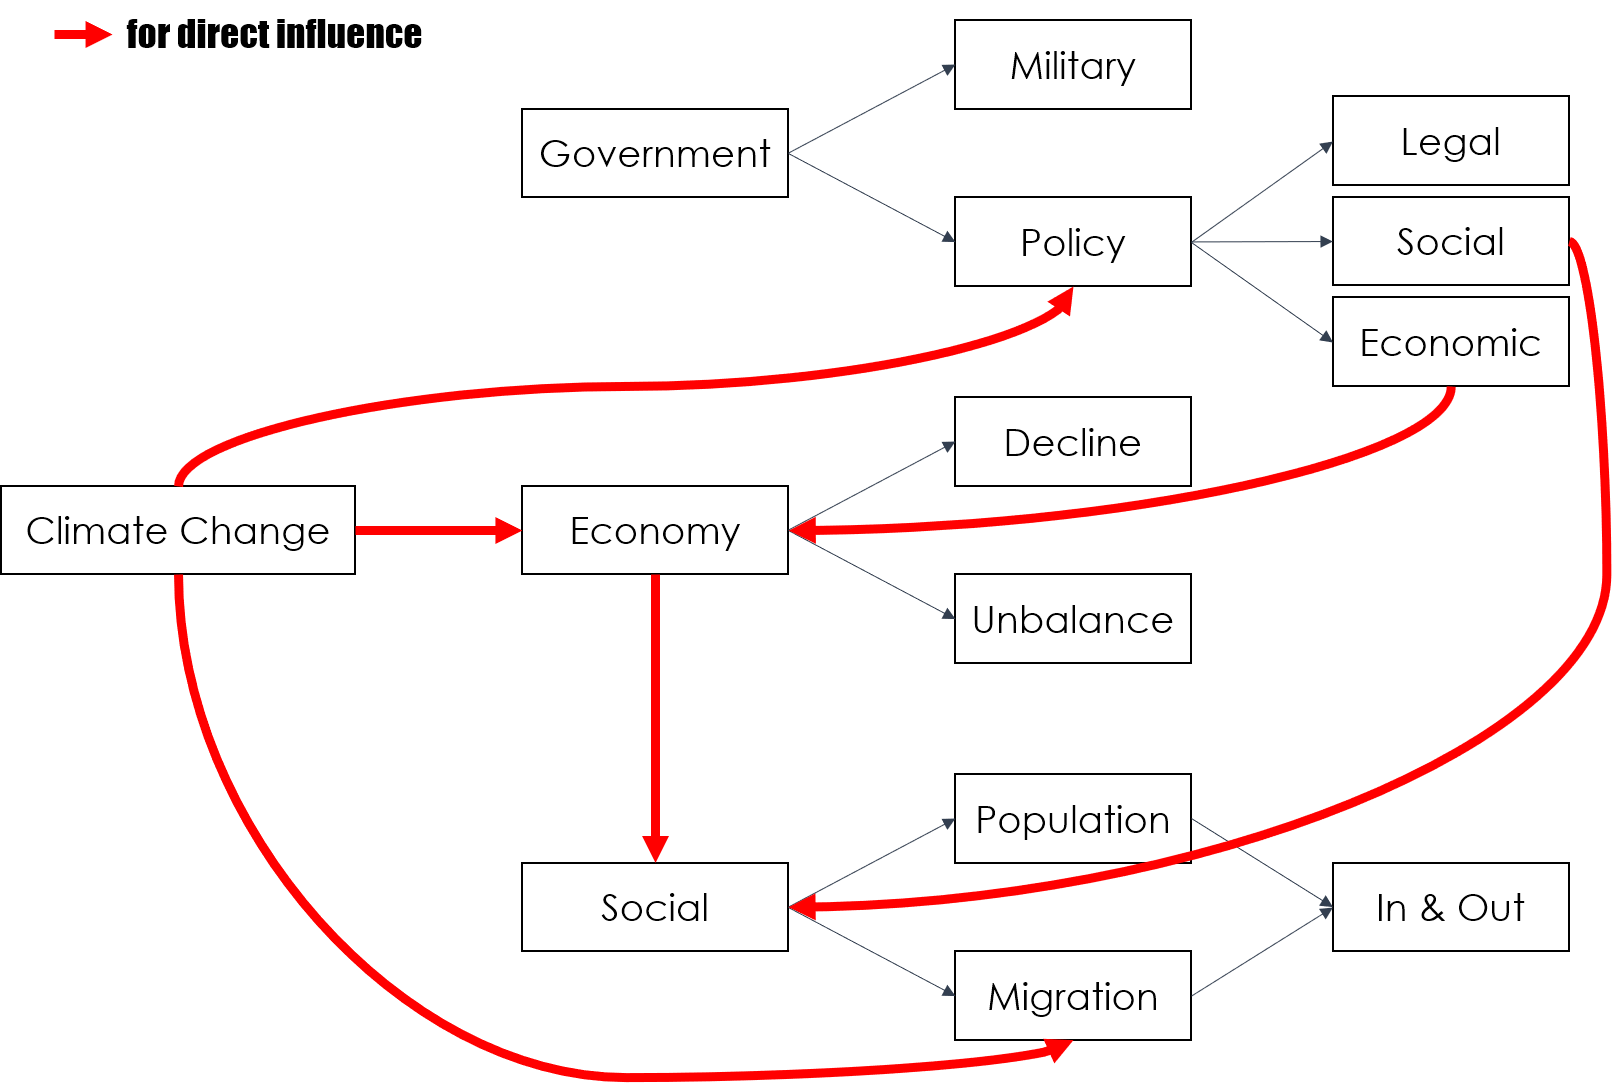
\includegraphics[width=14cm]{figure2.png}
		\caption{Stage-structured model of current process} \label{fig:Stage-structured model of current process}
	\end{figure}
	
	\noindent Additionally, the quantities involved in the function are shown in \textbf{Table 1} and \textbf{Table 2}. We list subscripts and primary notations apart.\\
	
	\begin{table}[htbp]
		\renewcommand\arraystretch{1.5}
		\footnotesize
		\centering
		\begin{tabular}{m{3cm}<{\centering}|m{10cm}<{\centering}}
			\whline
			\textbf{Subscript}&\textbf{Definition}\\
			\whline 
			$N$&$N_{th}$ year\\ 
			\shline
		\end{tabular}
		\caption{Definition of Subscripts in the model}\label{tab:Definition of Subscripts in the model}
	\end{table}
	\begin{table}[htbp]
		\renewcommand\arraystretch{1.5}
		\footnotesize
		\centering
		\begin{tabular}{m{3cm}<{\centering}|m{10cm}<{\centering}}
			\whline
			\textbf{Notation}&\textbf{Definition}\\
			\whline 
			$F$&Degree of Fragility\\
			$C$&Climate factor\\
			$E$&Economic factor\\
			$S$&Social factor\\
			$P$&Policy factor\\ 
			$M$&Military factor\\
			$X$&External Intervention\\
			\shline
		\end{tabular}
		\caption{Definition of notations in the model}\label{tab:Definition of notations in the model}
	\end{table}
	
	To evaluate the fragility of a country, we define the evaluation function $F$
	
	\begin{equation}
	F = w 
	\left(
	\begin{matrix}
	P_N \\ M_N \\ E_N \\ S_N
	\end{matrix}
	\right)
	\end{equation}
	
	In the function, $w$ is the weight of the variables, which is $(w_1, w_2, w_3, w_4)$. Since in the subsequent paragraphs we will normalize $P_N, M_N, E_N, S_N$, and for conciseness of the formula, we could assign w to be 1 for each variable.
	
	As assumed, if climate and external intervention remains zero, our major factors should be a \textbf{Markov Model}, which is
	
	$$
	\left(
	\begin{matrix}
	P_{N+1} \\ M_{N+1} \\ E_{N+1} \\ S_{N+1}
	\end{matrix}
	\right) 
	= 
	\left(
	\begin{matrix}
	k_{11} & k_{12} & k_{13} & k_{14} \\
	k_{21} & k_{22} & k_{23} & k_{24} \\
	k_{31} & k_{32} & k_{33} & k_{34} \\
	k_{41} & k_{42} & k_{43} & k_{44} \\
	\end{matrix}
	\right) 
	\left(
	\begin{matrix}
	P_N \\ M_N \\ E_N \\ S_N
	\end{matrix}
	\right) 
	$$
	Specifically, $P$ is the negative effect of improper policy issued by the government, $M$ is the decrease of security apparatus, $E$ is economic declining, and $S$ is social unrest. Assume coefficient matrix is $K$, then the function becomes
	$$
	\left(
	\begin{matrix}
	P_{N+1} \\ M_{N+1} \\ E_{N+1} \\ S_{N+1}
	\end{matrix}
	\right) 
	= 
	K
	\left(
	\begin{matrix}
	P_N \\ M_N \\ E_N \\ S_N
	\end{matrix}
	\right) 
	$$
	
	\subsection{Modified Markov Model including climate change}
	
	We can find in the schema (\textbf{Figure 1}) that climate change has direct influence on \textbf{policy factor}, \textbf{economy factor} and \textbf{social factor}, which indicates that there are several modifications to make. Since only the \textbf{military factor} is not affected, the modified prediction function should be as follow
	
	$$
	\left(
	\begin{matrix}
	P_{N+1} \\ M_{N+1} \\ E_{N+1} \\ S_{N+1}
	\end{matrix}
	\right) 
	= 
	K 
	\left(
	\begin{matrix}
	P_N \\ M_N \\ E_N \\ S_N
	\end{matrix}
	\right) 
	+
	K_c
	C
	, \quad
	K_c = 
	\left(
	\begin{matrix}
	k_{CP} \\ {0} \\ k_{CE} \\ k_{CS}
	\end{matrix}
	\right)
	$$
	$CP$ is the influence , There may be doubts whether \textbf{military factor} will be affected. As a matter of fact, \textbf{military factor} will change, but not on the direct effect of climate change. The indirect influence from climate change will appear while running the modified prediction function. For example, catastrophe causes social instability, then the military level changes, which might take some time for strategic planning.
	
	
	\subsection{Estimation for some parameters}
	Three effects of climate change (natural disasters, sea-level rise, and increasing resource scarcity) are frequently assumed to lead to loss of livelihood, economic decline, and increased insecurity either directly or through forced migration. Interacting with poor governance, societal inequalities, and a bad neighborhood, these factors in turn may promote
	political and economic instability, social fragmentation, migration, and inappropriate responses from governments. Eventually this produces increased motivation for instigating violence as well as improved opportunities for mobilization.[2]
	
	Events related to climate may cause a huge influence on the society, since they will impact the provisionment, conditions of countries and communities, and acquisition of clean water and energy. For example, according to a report from the Climate Action Network of Australia, climate change may decrease the precipitation of prairies, which may lead to a $15\%$ decline in grass productivity. In turn, it could further result in a $12\%$ drop in average weight of cattle, which decreases the beef supply. Under such condition, milk yield of cattle will decline by $30\%$, and new pests will spread in the areas. Furthermore, such condition will cause a $10\%$ decline of drinking water. According to the model of upcoming changing conditions, in the next 15 - 30 years, such situation may happen in a number of grain production bases around the world, which will result in an enormous impact on the economy and society to a large extent. 
	
	In addition, A long line of research links hot temperatures to individual aggression, including violent crime and riots. The simple scarcity (neo-Malthusian) model of conflict assumes that if climate change results in a reduction in essential resources for livelihood, such as food or water, those affected by the increasing scarcity may start fighting over the remaining resources. Alternatively, people may be forced to leave the area and create new scarcities when they encroach on the territory of other people who may also be resource-constrained. Barnett and Adger (2007) review a broad range of studies of both of these effects, focusing particularly on countries where a large majority of the population is still dependent on employment in the primary sector. If climate change results in reduced rainfall and higher temperature that jointly causes droughts, and reduced access to the natural capital that sustains livelihoods, poverty will be more widespread and the potential for conflict greater.[2]
	
	\begin{table}[htbp]
		\renewcommand\arraystretch{1.5}
		\footnotesize
		\centering
		\begin{tabular}{m{3.8cm}<{\centering}|m{4.8cm}<{\centering}|m{4.8cm}<{\centering}}
			\whline
			\textbf{Hypothesis}&\textbf{$P_N$}&\textbf{$M_N$}\\
			\whline
			\textbf{Abnormal precipitation}& 2 support, 1 none, 1 opposite &1 support, 2 none, 1 opposite\\
			
			\textbf{Abnormal temperature}&1 support, 2 none, 1 opposite&1 support, 1 none, 1 opposite\\
			
			\textbf{Natural disasters}&2 support, 1 opposite&1 none\\
			
			\textbf{Sea level rising}&2 support, 1 none, 1 opposite&1 support, 1 none, 1 opposite\\
			
			\textbf{Energy deficiency}&2 support, 1 opposite&3 none\\
			
			\textbf{Less vegetation}&2 none&1 none\\
			
			\shline
			\textbf{Hypothesis}&\textbf{$E_N$}&\textbf{$S_N$}\\
			\whline
			\textbf{Abnormal precipitation}& 3 support, 1 some support &2 support, 1 opposite\\
			
			\textbf{Abnormal temperature}&4 support, 1 none, 2 opposite&2 support, 1 none, 1 opposite\\
			
			\textbf{Natural disasters}&6 support, 1 opposite&6 support, 2 opposite\\
			
			\textbf{Sea level rising}&3 support, 1 none, 1 opposite&2 none\\
			
			\textbf{Energy deficiency}&2 support, 1 opposite&2 support, 1 none, 1 opposite\\
			
			\textbf{Less vegetation}&3 support, 1 none, 1 opposite&2 support, 1 opposite\\
			\shline
		\end{tabular}
		\caption{Influence of climate change - Quantitative study}\label{tab:Influence of climate change - Quantitative study}
	\end{table}
	
	\begin{table}[htbp]
		\renewcommand\arraystretch{1.5}
		\footnotesize
		\centering
		\begin{tabular}{m{2.7cm}<{\centering}|m{5cm}<{\centering}|m{5cm}<{\centering}}
			\whline
			\textbf{Hypothesis}&\textbf{$P_N$}&\textbf{$M_N$}\\
			\whline
			\textbf{$P_N$}&3 support &2 support, 1 none, 2 opposite\\
			
			\textbf{$M_N$}&2 support, 1 none, 2 opposite&4 support\\
			
			\textbf{$E_N$}&4 support, 1 none&1 support, 1 opposite\\
			
			\textbf{$S_N$}&1 support, 1 none&2 support, 1 none, 1 opposite\\
			\shline
			\textbf{Hypothesis}&\textbf{$E_N$}&\textbf{$S_N$}\\
			\whline
			\textbf{$P_N$}& 3 support, 1 none, 1 opposite & 1 support, 1 none\\
			
			\textbf{$M_N$}&1 support, 2 none&1 support, 1 none\\
			
			\textbf{$E_N$}&3 support&1 support, 2 none\\
			
			\textbf{$S_N$}&1 support, 2 none&1 support\\
			\shline
		\end{tabular}
		\caption{Interplay of different factors - Quantitative study}\label{tab:Interplay of different factors - Quantitative study}
	\end{table}
	
	We apply quantitative analysis on the influence of climate change (\textbf{Table 3}) and interplay of other factors (\textbf{Table 4}). The figures in each cell denote the number of studies that support, do not support, or contradict the proposed hypothesis. The total number of
	reviewed studies per outcome is computed and will be used for the computation of parameters. To be more specific, for each cell we need to calculate an parameter that represents the influence of the row factor on the column factor. If there is a study that supports the relation, we increase the outcome by 1; if there is a study that is opposite to the relation, we decrease it by 1. Then we calculates the sum of each row, and consider the proportion of each cell in the sum as the parameter of that cell. 
	
	Finally ,we attain matrix $K$ and $K_c$ as follows
	\begin{spacing}{1.5}
		$$
		K = 
		\left(
		\begin{matrix}
		\frac{1}{2} & 0 & \frac{1}{3} & \frac{1}{6} \\
		0 & \frac{2}{3} & \frac{1}{6} & \frac{1}{6} \\
		\frac{1}{2} & 0 & \frac{3}{8} & \frac{1}{8} \\
		\frac{1}{4} &\frac{1}{4} & \frac{1}{4} & \frac{1}{4} \\
		\end{matrix}
		\right) 
		, \quad K_c = 
		\left(
		\begin{matrix}
		\frac{1}{8} \\ {0} \\ \frac{1}{2} \\ \frac{1}{4}
		\end{matrix}
		\right) 
		$$
	\end{spacing}
	Therefore, the final prediction function becomes
	\begin{spacing}{1.5}
		\begin{equation}
		\left(
		\begin{matrix}
		P_{N+1} \\ M_{N+1} \\ E_{N+1} \\ S_{N+1}
		\end{matrix}
		\right) 
		= 
		\left(
		\begin{matrix}
		\frac{1}{2} & 0 & \frac{1}{3} & \frac{1}{6} \\
		0 & \frac{2}{3} & \frac{1}{6} & \frac{1}{6} \\
		\frac{1}{2} & 0 & \frac{3}{8} & \frac{1}{8} \\
		\frac{1}{4} &\frac{1}{4} & \frac{1}{4} & \frac{1}{4} \\
		\end{matrix}
		\right) 
		\left(
		\begin{matrix}
		P_N \\ M_N \\ E_N \\ S_N
		\end{matrix}
		\right) 
		+
		\left(
		\begin{matrix}
		\frac{1}{8} \\ {0} \\ \frac{1}{2} \\ \frac{1}{4}
		\end{matrix}
		\right) 
		C
		\end{equation}
	\end{spacing}	
	
	\subsection{Obtain fragility standard}
	It makes no sense to draw up standards out of an imaginary country, so we choose to investigate several countries which are widely accepted as stable, vulnerable and fragile.
	We respectively define Egypt, China and Italy to be fragile, vulnerable and stable, then we do research in Fragile States Index database(see the appendix) to calculate the policy factor, military factor, economy factor and social factor. Our factors are gained by 
	\begin{spacing}{1.5}
		\begin{equation}
		\begin{aligned}
		&P=\frac{1}{2}PS+\frac{1}{2}HR\\
		&M=SA\\
		&E=\frac{1}{3}EC+\frac{1}{3}UD+\frac{1}{3}HF\\
		&S=\frac{1}{2}DP+\frac{1}{2}RI\\
		\end{aligned}
		\end{equation}
	\end{spacing}
	
	The results are as follows (\textbf{Table 5})
	
	\begin{table}[htbp]
		\renewcommand\arraystretch{1.5}
		\footnotesize
		\centering
		\begin{tabular}{m{2cm}<{\centering}|m{2cm}<{\centering}|m{2cm}<{\centering}|m{2cm}<{\centering}|m{2cm}<{\centering}}
			\whline
			&\textbf{$P$}&\textbf{$M$}&\textbf{$E$}&\textbf{$S$}\\
			\whline
			\textbf{Italy}& 2.35 & 4.5 & 3.43 & 4.9\\
			
			\textbf{China}& 7.1 & 5.9 & 5.53 & 5.8\\
			
			\textbf{Egypt}& 7.35 & 8.1 & 6.3 & 7.2\\
			
			\shline
		\end{tabular}
		\caption{Factors of Italy, China and Egypt}\label{tab:Factors of Italy, China and Egypt}
	\end{table}
	After getting these data, we use the evaluation function $(1)$ to obtain their fragility. (\textbf{Table 6})
	
	\begin{table}[htbp]
		\renewcommand\arraystretch{1.5}
		\footnotesize
		\centering
		\begin{tabular}{m{2cm}<{\centering}|m{5cm}<{\centering}}
			\whline
			&\textbf{$F$}\\
			\whline
			\textbf{Italy} & 15.1833\\
			
			\textbf{China} & 24.33\\
			
			\textbf{Egypt} & 28.95\\
			
			\shline
		\end{tabular}
		\caption{Fragility of Italy, China and Egypt}\label{tab:Fragility  of Italy, China and Egypt}
	\end{table}
	
	So we can now define stable as fragility below 15.18, vulnerable as fragility above 24.33 and fragile as fragility above 28.95.
	
	\subsection{The Impact of Climate Change}
	
	In this section, we use an example to further illustrate the impact of climate change. Applying our model, we measure the impact of climate change and analyze how it changes the fragility of a state. We first assume the change of climate is random, and compare the fragility of the country with and without the influence of climate change. Then we assume the climate change is always negative, and do the same comparison.
	
	As is shown in \textbf{Figure 2},  calculated by our model above, the red line represents the fragility of the country as time passes without the influence of climate change; the green line is the fragility with the indirect influence of climate change; the blue line is the fragility with the indirect and direct influence of climate change. According to the figure, the impact of climate change has both positive and negative side. 
	\begin{figure}[h]
		\small
		\centering
		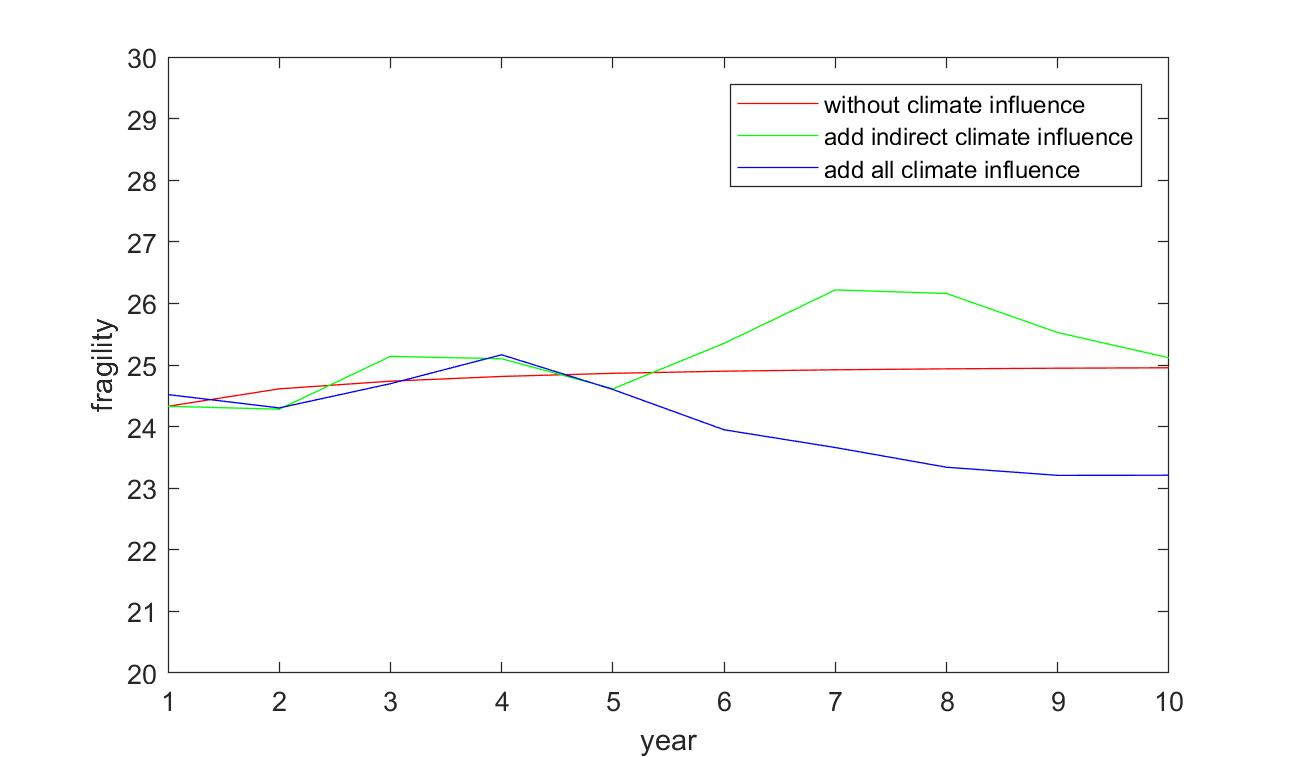
\includegraphics[width=14cm]{figure3.jpg}
		\caption{Fragility-Year Graph with random climate change} \label{fig:Fragility-Year with random climate change}
	\end{figure}

	In \textbf{Figure 3}, the implication of each line is same as what is illustrated above. It is clear that climate change increases fragility of the country. It will cause such consequence through direct impact and indirect means, which accords with the discussion in the previous chapters.
	\begin{figure}[h]
		\small
		\centering
		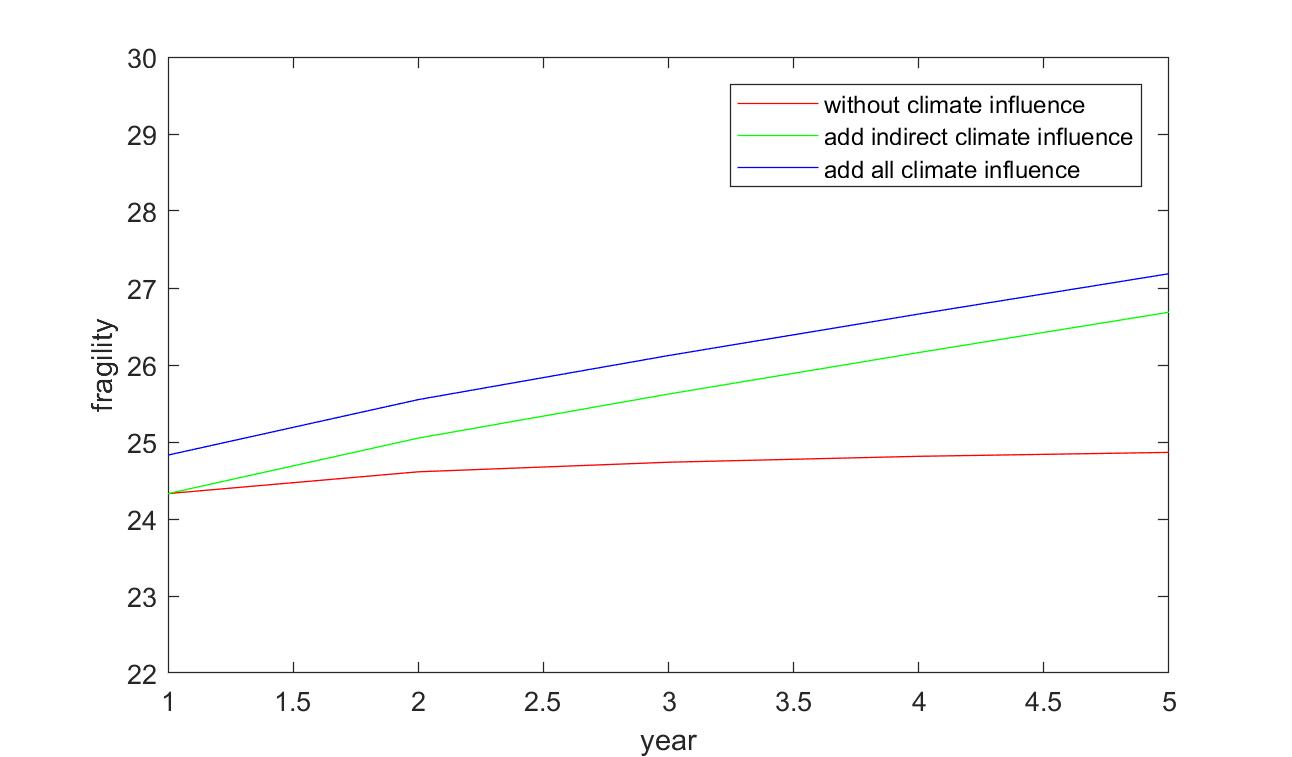
\includegraphics[width=13cm]{figure4.jpg}
		\caption{Fragility-Year Graph with negative climate change} \label{fig:Fragility-Year with random climate change}
	\end{figure}
	
	\section{Run model on the most fragile country}
	\subsection{How climate change increase fragility}
	In the section above, we have already build up our evaluation model of fragility. To test this model on some extreme situation, we first select one of the most fragile country: Central African Republic, which is on the edge of crashing. Its basic information are shown in \textbf{Table 7}

	\begin{table}[htbp]
		\renewcommand\arraystretch{1.5}
		\footnotesize
		\centering
		\begin{tabular}{m{2.5cm}<{\centering}|m{2.5cm}<{\centering}|m{2.5cm}<{\centering}|m{2.5cm}<{\centering}|m{2.5cm}<{\centering}}
			\whline
			\textbf{C1: Security Apparatus}&\textbf{C2: Factionalized Elites}&\textbf{C3: Group Grievance}&\textbf{E1: Economy}&\textbf{E2: Economic Inequality} \\
			\whline
			9.0 & 9.7 & 9.1 & 9.1 & 10.0\\
			\whline
			\textbf{E3: Human Flight and Brain Drain}&\textbf{P1: State Legitimacy}&\textbf{P2: Public Services}&\textbf{P3: Human Rights}&\textbf{S1: Demographic Pressures} \\
			\whline
			7.5 & 9.7 & 10.0 & 9.7 & 9.0\\
			\whline
			\textbf{S2: Refugees and IDPs}&\textbf{X1: External Intervention}&\textbf{Total}& \textbf{Rank} & \\
			\whline
			10.0 & 9.8 & 112.6 & 3rd &\\
			\shline
		\end{tabular}
		\caption{Info of Central African Republic in 2017}\label{tab:Info of Central African Republic in 2017}
	\end{table}
	
	
	In the Fragile States Index data base, we can find some major factors for our model. After data conversion, we obtain the inputs for our prediction function (\textbf{Table 8})
	
	\begin{table}[htbp]
		\renewcommand\arraystretch{1.5}
		\footnotesize
		\centering
		\begin{tabular}{m{2.5cm}<{\centering}|m{2.5cm}<{\centering}|m{2.5cm}<{\centering}|m{2.5cm}<{\centering}}
			\whline
			\textbf{$P$}&\textbf{$M$}&\textbf{$E$}&\textbf{$S$}\\
			\whline
			9.85 & 9 & 8.87 & 9.5 \\
			\shline
		\end{tabular}
		\caption{Factors of Central African Republic}\label{tab:Factors of Central African Republic}
	\end{table}
	
	First, we want to determine how climate change may have increased fragility of Central African Republic, which is similar to what we have done in the last section. We assume the climate change to be a constant negative factor. The fragility of Central African Republic in 5 years is shown below
	
	\begin{figure}[h]
		\small
		\centering
		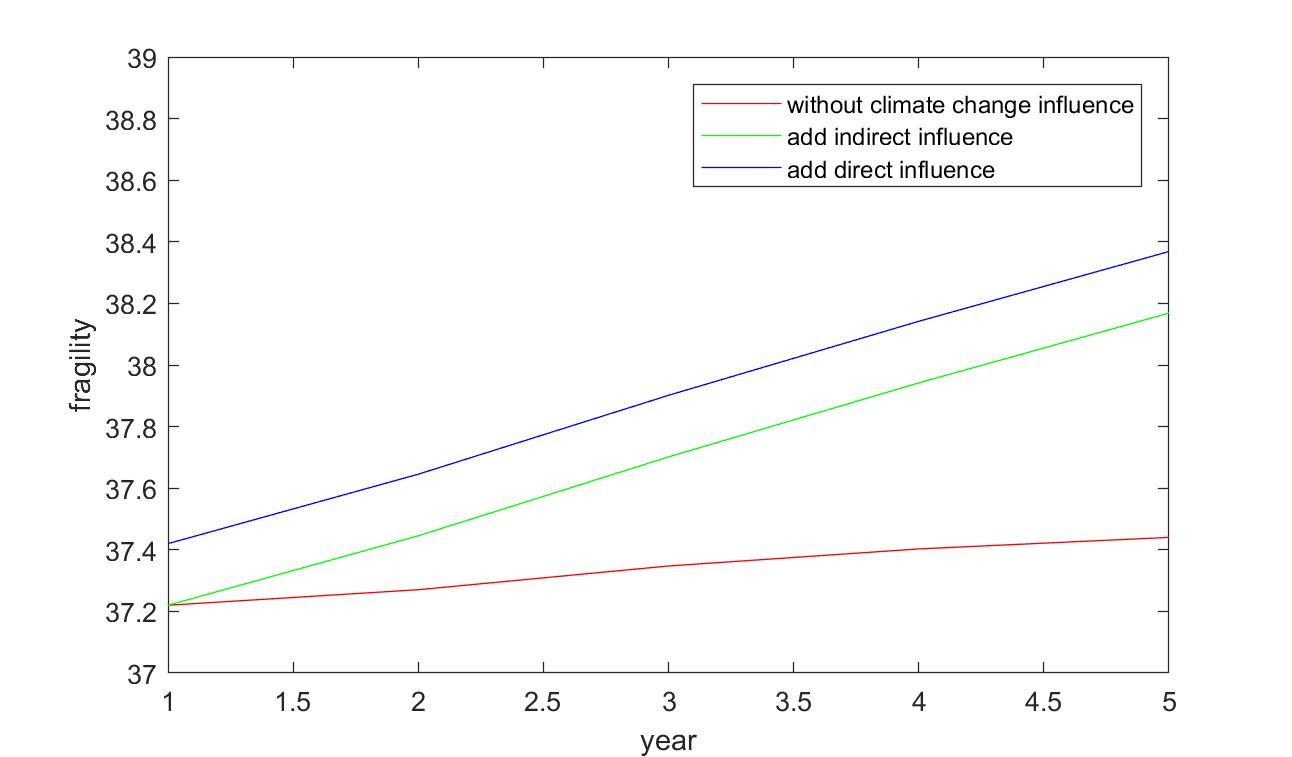
\includegraphics[width=15cm]{figure5.jpg}
		\caption{Fragility-Year Graph of Central African Republic} \label{fig:Fragility-Year Central African Republic}
	\end{figure}
	
	It is apparent that if climate continue to be negative, a country will find it hard to adjust its policy, economy and society to reduce fragility. The fragility of Central African Republic is high enough in 2017, which can be even worse if climate remains harmful.


	\subsection{Ways to mitigate fragility}
	Then we try to find the fragility trend without climate change factor. Among the four factors we defined, policy factor is the only one that government can control, others can only be affected by the policy factor. So, we set climate factor to 0 and change policy factor, trying to find the value of policy factor when fragility won’t get worse in 5 years.
	
	Below is the fragility changing curve when policy factor is down to 9.37, the fragility will get better in 2 years then adjust itself to become as fragile as before, which indicate that in this kind of country, positive policy may not last long in current situation.
	
	\begin{figure}[h]
		\small
		\centering
		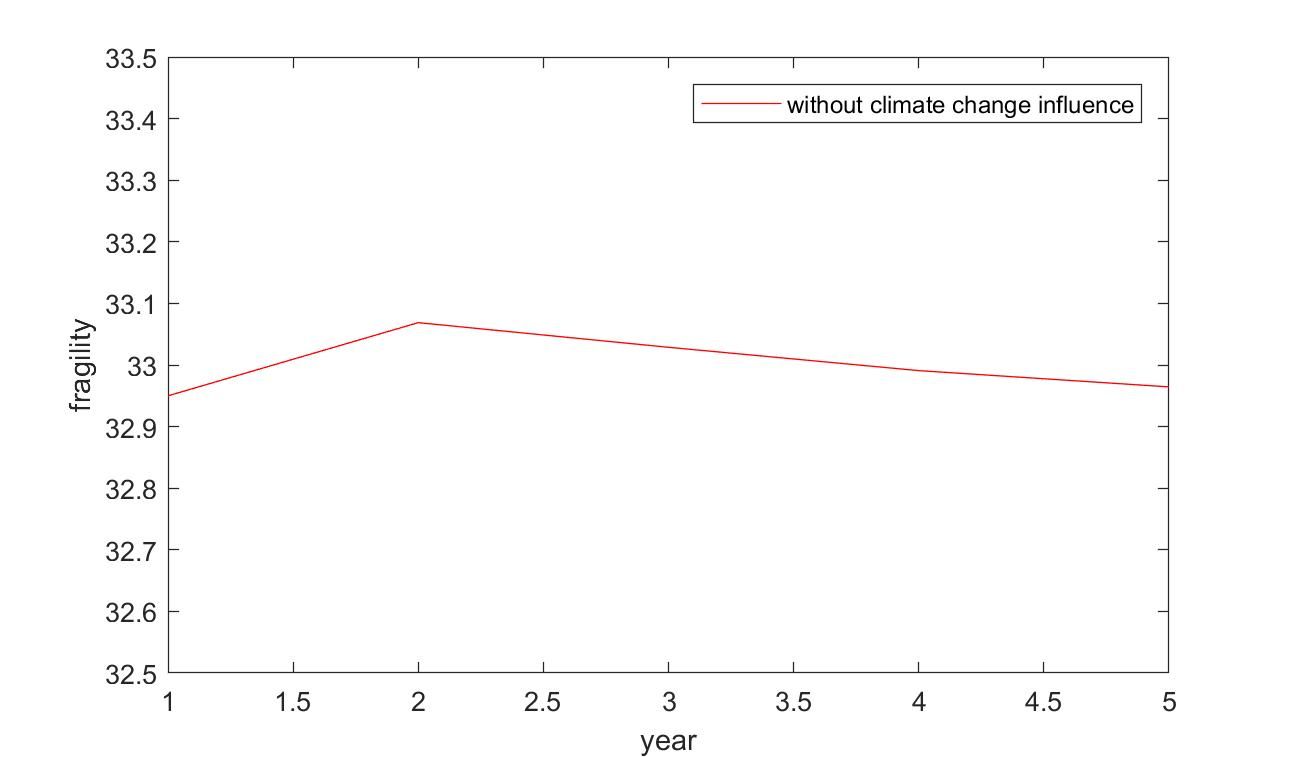
\includegraphics[width=15cm]{figure6.jpg}
		\caption{Fragility-Year of Graph Central African Republic} \label{fig:Fragility-Year Central African Republic}
	\end{figure}
	
	So, the conclusion can be drawn: If government can still make right, positive decisions on economic and social policies, then the fragility might not get higher. If this country wants to be less fragile, its government should be very capable and outstanding on making right decisions, which might not be the case in most fragile countries.

	\section{Run model on the stable country}
	\subsection{Refine model with more specific climate change}
	In this chapter, we choose countries with high stability for data analysis, since such countries have dramatic difference with countries involved in the previous discussion. Furthermore, the choice of country will affect our choice of climate parameters. For example, if we choose landlocked countries, the impact of sea-level rise should not be a major factor.
	
	Select a specific N as iteration time. Assume each climate factor is $C_i$, the corresponding weight is $k_{c_i}$.  We iterate under the constraint condition that the fragility of a state does not increase. Therefore, we have the following equation
	
	$$
	\Sigma k_{c_i} C_i \leq const
	$$
	
	The weight assigned to each factor reflects the degree of influence of the corresponding climate factor on the fragility of a country.
	
	In practice, we select the Netherlands to calculate the impact of the climate. After researching on the national conditions in the Netherlands, we find that climate factors that have a major impact on the fragility of the Netherlands include: anomalies in temperature ($T$), anomalies in rainfall ($R$), sea-level rise ($L$) and natural disasters ($D$), which have significant influence on policy, military, economic and social factors. We can write the influence matrix and the vector of climate factor as follows:
	
	$$
	\left(
	\begin{matrix}
	P_{N+1} \\ M_{N+1} \\ E_{N+1} \\ S_{N+1}
	\end{matrix}
	\right) 
	= 
	K 
	\left(
	\begin{matrix}
	P_N \\ M_N \\ E_N \\ S_N
	\end{matrix}
	\right) 
	+
	K_c
	\left(
	\begin{matrix}
	D \\ L \\ P \\ S \\
	\end{matrix}
	\right)
	, \quad
	K_c = 
	\left(
	\begin{matrix}
		k_{c_{11}} & k_{c_{12}} & k_{c_{13}} & k_{c_{14}} \\
		k_{c_{21}} & k_{c_{22}} & k_{c_{23}} & k_{c_{24}} \\
		k_{c_{31}} & k_{c_{32}} & k_{c_{33}} & k_{c_{34}} \\
		k_{c_{41}} & k_{c_{42}} & k_{c_{43}} & k_{c_{44}} \\
	\end{matrix}
	\right)
	$$

	\subsection{Run model on the Netherlands}
	We select $N = 5$ as iteration time, and attain the equation that could satisfy the constrain condition:
	$$
	8.96D + 0.22E + 2.24L - 0.41M + 0.52P + 5.31R - 0.33S + 3.49T\leq0
	$$
	After assigning the data of the Netherlands in Fragile States Index data base, we can attain
	$$
	8.96D + 2.24L + 5.31R + 3.49T - 0.58\leq0
	$$
	The figures of this equation are shown in \textbf{Figure 6}.
	
	\begin{figure}[h]
		\small
		\centering
		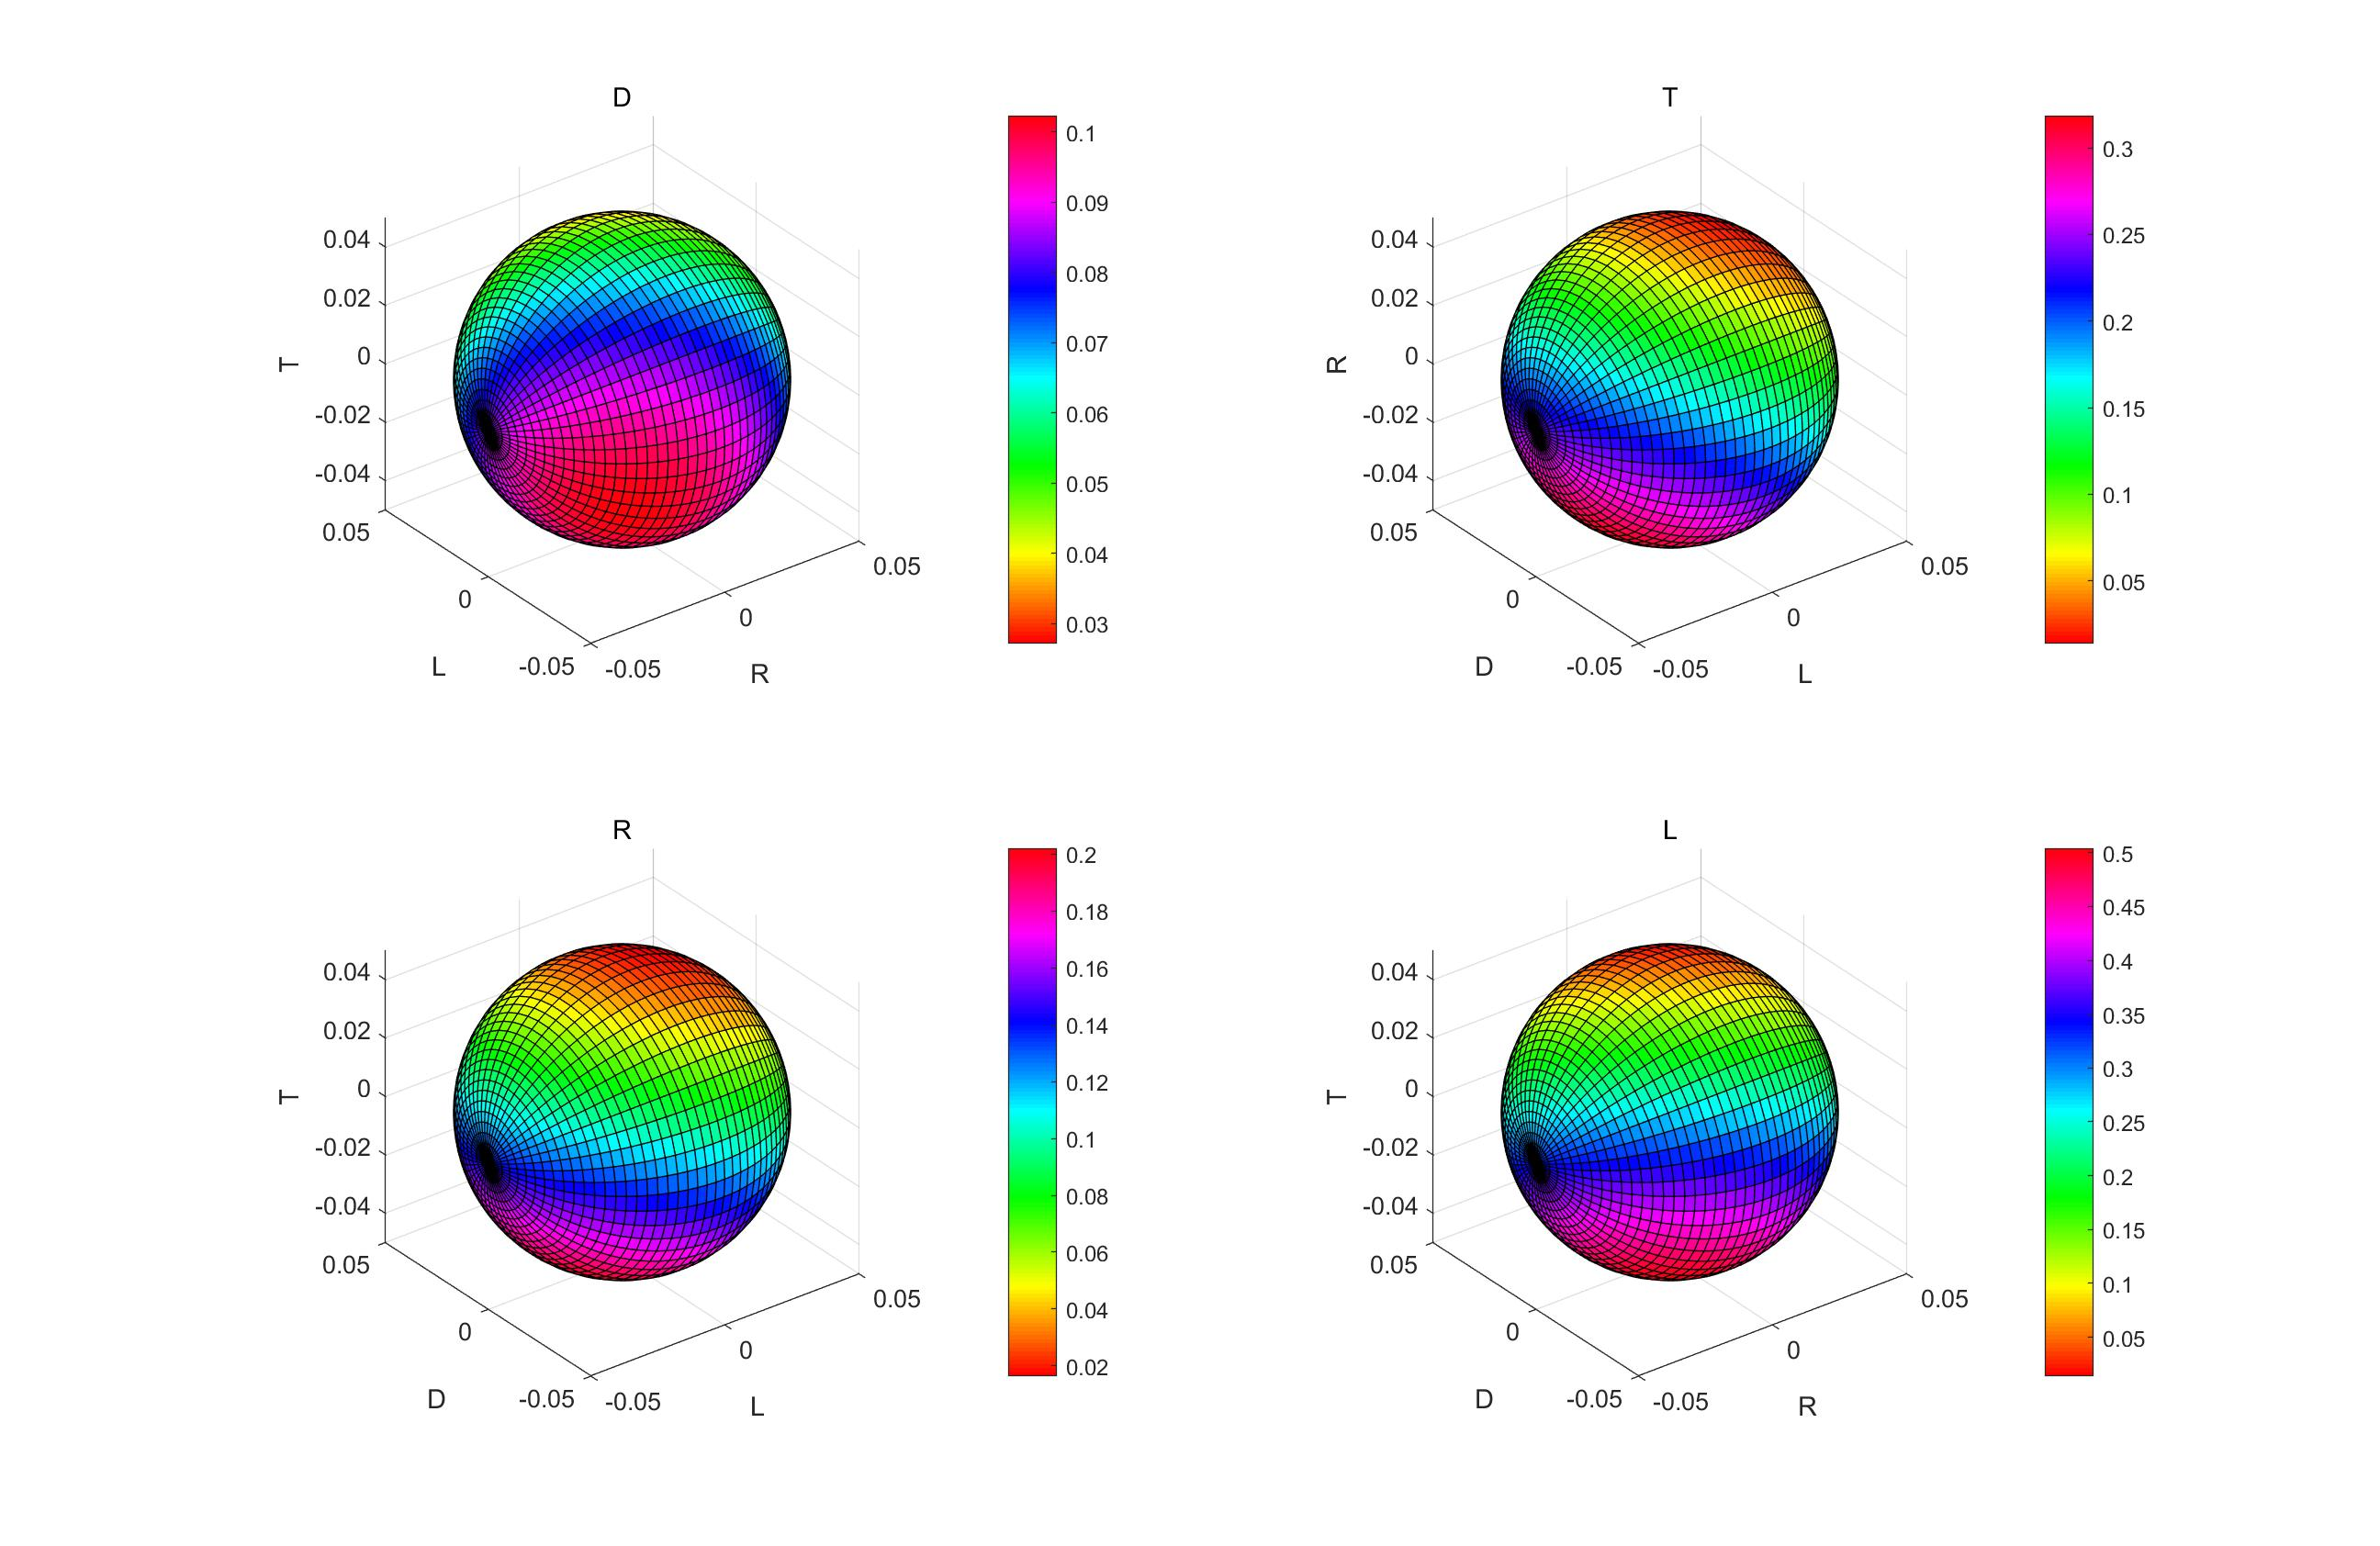
\includegraphics[width=16cm]{figure7.jpg}
		\caption{Figure of Climate Equation} \label{fig:Figure of Climate Equation}
	\end{figure}
	
	When the equation cannot be satisfied, which means the impact of climate change goes beyond the capacity of the Netherlands to regulate and control, the Netherlands will become more fragile within five years.
	The tipping point is when the climate change in the Netherlands satisfies
	$$
	8.96D + 2.24L + 5.31R + 3.49T - 0.58 = 0
	$$
	
	
	It can be seen that these climate factors have different effects on whether the equation can be satisfied, according to their coefficients in the equation. Natural disasters have the greatest influence. In another word, it is really difficult to completely avoid loss through various policies when serious natural disasters occur. In addition,  the sea-level rise has relatively less impact on the Netherlands. In practice, however, natural disasters in the Netherlands occur less frequently, while sea-level rise is a constant threat to the Netherlands due to the low elevation and can easily affect social stability by causing massive immigration and declining social order. So if we want to get a universal and complete evaluation of a country, we also need to investigate the various climate factors in the country and the frequency and duration of their occurrence.
	
	\section{Policy and recommendations}
	\begin{itemize}
		\item Based on the model established primitively, the speed of document check is twice over that of screening, as a consequence, the screening process contributes most to the appearance of bottlenecks. Therefore, the airport should dispatch more skilled TSA officers to the screening area and expedite the speed of screening.
		\item Rationally arrange the number of entrances and lanes. From the optimization we have made, the best arrangement is shown below
		$$N_X:N_B=2:1$$
		$$\lambda_P:\lambda_R=3:2$$
		$$N_X=1.2(N_P+N_R)$$
		\item Monitor the flow of passengers in real time, and arrange the number of entrances according to the acquired values in order to reduce the cost on the basis of rational efficiency. The optimal result we obtain according to data we have is
		$$s=\lceil\frac{\lambda}{\mu}-0.5\rceil+1$$
		\item Arrange different number of TSA officers and security staffs in different security checkpoints in order to adjust the average waiting time of passengers. For instance, in the checkpoints with more queue-jumpers, we should arrange more staffs to insure that disputes caused by cutting will not continue for a long period. In the sensitivity analysis, the increasing velocity of queues satisfy that
		$$\frac{dL_q}{dt}=\frac{\lambda s_{paralyzed}}{s(s-s_{paralyzed})}$$
		We assumed that all kinds of disputes will be solved in five minutes, and if such time increases, the queue will be so long that passengers may suffer from anxiety.
		\item Promote Pre-Check service, and increase the number of Pre-Check entrances, which will provide convenience to passengers and save the checking time. It is mentioned that 45\% of passengers enroll in Pre-Check, but since Pre-Check passengers tend to travel more frequently by plane, such proportion cannot be the criterion when deciding the number of Pre-Check entrances and regular entrances.
		\item Establish a baggage buffer that used to temporarily store the baggage that has been checked. Since in our optimization each lane for body screening is accompanied with two lanes for baggage screening, which will increase the probability of baggage checked faster than passengers, such buffer can prevent the occurrence of congestion and improve the security level of baggage.
		\item In the sensitivity analysis, we find that culture discrepancies will not impact greatly the queuing time, and the existing congestion mainly due to the insufficiency of entrances. Therefore, we propose that if cost permitting, the airport should open more entrances and disperse entrances as much as possible in order to disperse passengers, which will relief the anxiety of them.
	\end{itemize}
	\section{Strengths and weaknesses}
	\subsection{Strengths}
	\begin{itemize}
		\item Our model separates the whole process of security check into ID-check part and screening part, and independently calculates the corresponding queuing conditions, which avoid the possible errors due to the complicated model.
		\item We estimate the arrival rate for each passenger and the checking time for each TSA officer, and assume that the former obeys Poisson Distribution and the latter obeys Exponential Distribution, which conform to the general principles.
		\item We apply the moment estimation to estimate relevant parameters of the system so as to obtain the basic model.
		\item We apply the Queuing Theory, and consider the average waiting time and the flow of passengers as our principal evaluation indexes, which correspond with profits of airports and passengers.
		\item When analyzing the sensitivity and improving the current model, we consider the difference of average waiting time and the maximal flow of passengers as our principal evaluation indexes, which guarantee that the airport can provide every passengers with the approximately same service with the maximal efficiency.
	\end{itemize}
	\subsection{Weaknesses}
	\begin{itemize}
		\item Since we do not have enough data, we have to estimate related parameters using moment estimation of data given. The error can be large when the data size is small.
		\item The bound between service time and waiting time is not explicit enough. We assume that when passengers put their baggage on the belt, they finish waiting and service time begins, but actually perhaps passengers consider the time between the moment they put down their baggage and the moment they receive body screening is also the waiting time.\item Since we have less estimation of costs and utilization of space, our model considers efficiency and flying experience of passengers as the principal indexes. In fact, we should modify our model according to actual costs of airport construction.
		\item We did not take the scale of the airport into account, and modeling based on the given data. If the scale of the airport is large enough, we need to rewrite some of our codes to obtain a more graceful result.
	\end{itemize}
	
	\begin{thebibliography}{99}
		\bibitem{1}\url{https://en.wikipedia.org/wiki/Fragile_state#Defining_fragile_states}
		\bibitem{2}Schwartz, P. and Randall, D. “An Abrupt Climate Change Scenario and Its Implications for United States National Security”, October 2003.
		\bibitem{3}Clara V. Marin, Colin G. Drury, Rajan Batta, Li Lin. Server Adaptation in an Airport Security System Queue[J].The OR Society, 2007, Vol.20:22-31.
		\bibitem{4}Zeng Junjie. Optimization and Configuration of Airport Security. Wide Angle, 2009:173-174.
		\bibitem{5}MI Kamien,NL Schwartz. Dynamic Optimization: The Calculus of Variations and Optimal Control in Economics \& Management.North Holland, 1981, 31(1):1252-1257.
		\bibitem{6}Zhang Guofen, Huang B Q, Zhang C Y. Probability Theory, Mathematical Statistics and Stochastic Process. Zhejiang University Press, 2011.
		\bibitem{7}Ivo Adan, Jacques Resing. Queueing Systems.Department of Mathematics and Computing Science Eindhoven University of Technology, P.O. Box 513, 5600 MB Eindhoven, The Netherlands, 2015.
		\bibitem{8}Queueing theory (https://en.wikipedia.org/wiki/Queueing\_theory).
	\end{thebibliography}
	
	\begin{appendices}
		
		\section{First appendix}
		Here are data  about how passengers proceed through each step of the security screening process. \\

		
		
		
		
		
		
		
		
		\section{Second appendix}
		Here are simulation programmes we used in our model as follow.
		\noindent \textbf{\textcolor[rgb]{0.98,0.00,0.00}{Draw the figure of $f_{omax}$ and $N_L/N_P$}}
		\lstinputlisting[language=Matlab]{./code/find_CARequal5.m}
%		\textbf{\textcolor[rgb]{0.98,0.00,0.00}{Find the zero point of the function $test$ }}
%		\lstinputlisting[language=Matlab]{./code/drive_test.m}
%		\textbf{\textcolor[rgb]{0.98,0.00,0.00}{Calculate $W_q$ for every specific $s$}}
%		\lstinputlisting[language=Matlab]{./code/test.m}
%		\textbf{\textcolor[rgb]{0.98,0.00,0.00}{Draw figures of $s$ and $\lambda$ when approaches to rounding $s$ are different}}
%		\lstinputlisting[language=Matlab]{./code/s_lambda1.m}
%		\textbf{\textcolor[rgb]{0.98,0.00,0.00}{Draw figures of $W_q$ and $\lambda$ when approaches to rounding $s$ are different}}
%		\lstinputlisting[language=Matlab]{./code/Wq_lambda1.m}
%		\textbf{\textcolor[rgb]{0.98,0.00,0.00}{Draw figures of $s$ and $\lambda$ when screening time is longer}}
%		\lstinputlisting[language=Matlab]{./code/s_lambda2.m}
%		\textbf{\textcolor[rgb]{0.98,0.00,0.00}{Draw figures of $W_q$ and $\lambda$ when screening time is longer}}
%		\lstinputlisting[language=Matlab]{./code/Wq_lambda2.m}
%		\textbf{\textcolor[rgb]{0.98,0.00,0.00}{Draw figures of $s$ and $\lambda$ when there are more passengers entering Zone D}}
%		\lstinputlisting[language=Matlab]{./code/s_lambda3.m}
%		\textbf{\textcolor[rgb]{0.98,0.00,0.00}{Draw figures of $W_q$ and $\lambda$ when there are more passengers entering Zone D}}
%		\lstinputlisting[language=Matlab]{./code/Wq_lambda3.m}
%		\noindent \textbf{\textcolor[rgb]{0.98,0.00,0.00}{Draw the figure of $dW_q/dt-\lambda$ when there is one entrance paralyzed}}
%		\lstinputlisting[language=Matlab]{./code/OneEntranceParalyzed.m}
%		\textbf{\textcolor[rgb]{0.98,0.00,0.00}{Draw the figure of $dW_q/dt-\lambda$ when there are two entrances paralyzed }}
%		\lstinputlisting[language=Matlab]{./code/TwoEntranceParalyzed.m}
	\end{appendices}
\end{document}

%% 
%% This work consists of these files mcmthesis.dtx,
%%                                   figures/ and
%%                                   code/,
%% and the derived files             mcmthesis.cls,
%%                                   mcmthesis-demo.tex,
%%                                   README,
%%                                   LICENSE,
%%                                   mcmthesis.pdf and
%%                                   mcmthesis-demo.pdf.
%%
%% End of file `mcmthesis-demo.tex'.